\documentclass{article}
\renewcommand{\baselinestretch}{1.25}

\usepackage{xeCJK}  % support character

% monokai code
\usepackage{color}
\usepackage{minted}
\usemintedstyle{manni}
\setminted{
    linenos,
    fontsize=\footnotesize,
    resetmargins
}

% insert images
\usepackage{graphicx}
\graphicspath{{images/}{../images/}}
\usepackage{amsmath}
\usepackage{caption}
\numberwithin{figure}{section}
\numberwithin{table}{section}
\numberwithin{listing}{section}
\numberwithin{equation}{section}

\usepackage{subcaption}

% hyperlink
\usepackage{hyperref}
\usepackage{xcolor}
\hypersetup{
    colorlinks,
    linkcolor={red!50!black},
    citecolor={blue!50!black},
    urlcolor={blue!80!black}
}

% auto newline in table
\newcommand{\tabincell}[2]{\begin{tabular}{@{}#1@{}}#2\end{tabular}}
\usepackage{multirow}

\usepackage{mathtools}
\usepackage{amsfonts}

\author{郭一隆(2013011189)}
\title{图像处理实验报告}

\begin{document}
    \maketitle

    \tableofcontents
    \newpage

    \listoffigures
    \listoftables
    \renewcommand\listoflistingscaption{List of Source Codes}
    \listoflistings
    \newpage

    \section{基础知识} % (fold)
    \label{sec:基础知识}

        在\texttt{MATLAB}中,像素值用\texttt{uint8}类型表示,参与浮点数运算前需要转成\texttt{double}型。Section \ref{sec:基础知识} 中“测试图像”指的是\href{run:../resource/hall.mat}{\texttt{hall.mat}}中的\textbf{彩色图像}。

        \begin{enumerate}
            \item \texttt{MATLAB}提供了图像处理工具箱,在命令窗口输入\texttt{help images}可查看该工具箱内的所有函数。请阅读并大致了解这些函数的基本功能。

                \begin{table}[H]
                    \caption{图像处理工具箱函数概览(部分)}
                    \label{tab:help_images}
                    \centering
                
                    \begin{tabular}{l|l}
                    \hline
                
                    \hline
                    \textbf{函数名} & \textbf{功能} \\
                    \hline
                        \texttt{imshow} & 在\texttt{figure}中显示图像 \\
                    \hline
                        \texttt{rgb2gray} & 将彩色图像转换为灰度值图像 \\
                    \hline
                        \texttt{imwrite} & 将图像矩阵写入文件 \\
                
                    \hline
                    \end{tabular}
                \end{table}

            \item 利用\texttt{MATLAB}提供的\texttt{Image file I/O}函数分别完成以下处理:
                \begin{enumerate}
                    \item 以测试图像的中心为圆心,图像的长和宽中较小值的一半为半径画一个\textcolor{red}{红颜色}的圆;

                        \textbf{思路:}利用\texttt{meshgrid}函数生成行列索引矩阵\texttt{I, J},将圆内部的像素点标为\textbf{逻辑1},再利用逻辑索引将测试图像圆内的部分替换为\textcolor{red}{红色像素点}。

                        \begin{listing}[H]
                            \caption{\texttt{draw\_circle.m}}
                            \label{listing:draw_circle}
                            \inputminted{matlab}{../draw_circle.m}
                        \end{listing}

                        \begin{figure}[H]
                            \centering
                                \begin{subfigure}{0.5\textwidth}
                                    \centering
                                    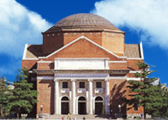
\includegraphics[width=0.4\linewidth]{hall_color}
                                    \caption{处理前}
                                    \label{fig:hall_color}
                                \end{subfigure}%
                                \begin{subfigure}{0.5\textwidth}
                                    \centering
                                    
\includegraphics[width=0.4\linewidth]{hall_color_red_circle}
                                    \caption{处理后}
                                    \label{fig:hall_color_red_circle}
                                \end{subfigure}

                            \caption{在大礼堂中心绘制红圆}
                            \label{fig:red_circle}
                        \end{figure}

                    \item 将测试图像涂成国际象棋状的“黑白格”的样子,其中“黑”即黑色,“白”则意味着\textbf{保留原图}。

                        \textbf{思路:}\texttt{chess\_mask}函数提供棋盘行列数接口,计算出每块的大小,同样利用\texttt{meshgrid}函数确定出\texttt{black\_mask}的位置,将图像对应位置赋为黑色。

                        \begin{listing}[H]
                            \caption{\texttt{chess\_mask.m}}
                            \label{listing:chess_mask}
                            \inputminted{matlab}{../chess_mask.m}
                        \end{listing}

                        按如下代码生成\texttt{64}格和\texttt{32}格棋盘蒙版

                        \begin{minted}{matlab}
>> imwrite(chess_mask(hall_color,8,8),'images/hall_color_masked_8_8.png')
>> imwrite(chess_mask(hall_color,4,8),'images/hall_color_masked_4_8.png')
                        \end{minted}

                        \begin{figure}[H]
                            \centering
                                \begin{subfigure}{0.5\textwidth}
                                    \centering
                                    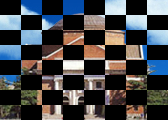
\includegraphics[width=0.4\linewidth]{hall_color_masked_8_8}
                                    \caption{$8\times8$蒙版}
                                    \label{fig:hall_color_masked_8_8}
                                \end{subfigure}%
                                \begin{subfigure}{0.5\textwidth}
                                    \centering
                                    
\includegraphics[width=0.4\linewidth]{hall_color_masked_4_8}
                                    \caption{$4\times8$蒙版}
                                    \label{fig:hall_color_masked_4_8}
                                \end{subfigure}

                            \caption{国际象棋蒙版}
                            \label{fig:chess_mask}
                        \end{figure}

                \end{enumerate}

                用看图软件浏览上述生成图片,预览效果如图\ref{fig:red_circle}和图\ref{fig:chess_mask},达到预期效果。

        \end{enumerate}
    
    % section 基础知识 (end)

    \section{图像压缩编码} % (fold)
    \label{sec:图像压缩编码}

        \textbf{熵编码压缩比}:

        根据经验,对于文本文件,重复性越高,则压缩比越高,测试如下表

        \begin{table}[H]
            \caption{WinRar压缩文本文件}
            \label{tab:winrar}
            \centering
        
            \ttfamily
            \begin{tabular}{l|l|l|l|l}
            \hline
        
            \hline
            \textbf{文件名} & \textbf{文本内容(matlab写入文件)} & \textbf{压缩前大小} & \textbf{压缩后大小} & \textbf{压缩比} \\
            \hline
                high.txt & repmat(['1'],1,10000) & 10000bytes & 101bytes & 99.01 \\
            \hline
                normal.txt & int2str(2\^{}1000) & 302bytes & 106bytes & 2.85 \\
            \hline
                low.txt & 'ghjkl;' & 6bytes & 77bytes & 0.08 \\
        
            \hline
            \end{tabular}
        \end{table}

        本章练习题所用数据均可由“JpegCoeff.mat”导入,其内容如表\ref{tab:JpegCoeff}所示。本章练习题中“测试图像”指的是\href{run:../resource/hall.mat}{\texttt{hall.mat}}中的\textbf{灰度图像}。

        \begin{table}[H]
            \caption{\texttt{JpegCoeff.mat}中所含数据}
            \label{tab:JpegCoeff}
            \centering
        
            \begin{tabular}{ccc}
            \hline
        
            \hline
            \textbf{变量名} & \textbf{含义} & \textbf{说明} \\
            \hline
                \texttt{QTAB} & \tabincell{l}{\texttt{DCT}系数的量化 \\步长矩阵,式(\ref{eq:QTAB})} & \\
            \hline
                \texttt{DCTAB} & \tabincell{l}{\texttt{DC}系数预测误差 \\的\texttt{Category}码本,\\表\ref{tab:DC_Huffman}} & \tabincell{l}{每行对应一个\texttt{Category},第一列对应\texttt{Huffman}编码 \\的长度\texttt{L},随后\texttt{L}列对应该码字,再后全零为填充物} \\
            \hline
                \texttt{ACTAB} & \tabincell{l}{\texttt{AC}系数的 (\texttt{Run/Size})\\的码本,完整的表\ref{tab:AC_Huffman}} & \tabincell{l}{每行对应一个(\texttt{Run/Size}),第一列表示\texttt{Run},第二列 \\表示\texttt{Size},第三列表示该(\texttt{Run/Size})对应的\texttt{Huffman} \\编码的长度\texttt{L},随后\texttt{L}列对应该码字,再后全零为填充物} \\
            \hline

            \hline
            \end{tabular}
        \end{table}

        \begin{equation}
        \label{eq:QTAB}
            Q = \left[
            \begin{matrix}
                16 & 11 & 10 & 16 & 24 & 40 & 51 & 61 \\
                12 & 12 & 14 & 19 & 26 & 58 & 60 & 55 \\
                14 & 13 & 16 & 24 & 40 & 57 & 69 & 56 \\
                14 & 17 & 22 & 29 & 51 & 87 & 80 & 62 \\
                18 & 22 & 37 & 56 & 68 & 109 & 103 & 77 \\
                24 & 35 & 55 & 64 & 81 & 104 & 113 & 92 \\
                49 & 64 & 78 & 87 & 103 & 121 & 120 & 101 \\
                72 & 92 & 95 & 98 & 112 & 100 & 103 & 99
            \end{matrix}
            \right]
        \end{equation}

        \begin{table}[H]
            \caption{亮度直流分量预测误差的\texttt{Category}及其\texttt{Huffman}编码}
            \label{tab:DC_Huffman}
            \centering
        
            \begin{tabular}{ccc}
            \hline
        
            \hline
            \textbf{预测误差} & \textbf{\texttt{Category}} & \textbf{\texttt{Huffman}编码} \\
            \hline
                0 & 0 & 00 \\
                -1, 1 & 1 & 010 \\
                -3, -2, 2, 3 & 2 & 011 \\
                -7, $\cdots$, -4, 4, $\cdots$, 7 & 3 & 100 \\
                -15, $\cdots$, -8, 8, $\cdots$, 15 & 4 & 101 \\
                -31, $\cdots$, -16, 16, $\cdots$, 31 & 5 & 110 \\
                -63, $\cdots$, -32, 32, $\cdots$, 63 & 6 & 1110 \\
                -127, $\cdots$, -64, 64, $\cdots$, 127 & 7 & 11110 \\
                -255, $\cdots$, -128, 128, $\cdots$, 255 & 8 & 111110 \\
                -511, $\cdots$, -256, 256, $\cdots$, 511 & 9 & 1111110 \\
                -1023, $\cdots$, -512, 512, $\cdots$, 1023 & 10 & 11111110 \\
                -2047, $\cdots$, -1024, 1024, $\cdots$, 2047 & 11 & 111111110 \\
            \hline

            \hline
            \end{tabular}
        \end{table}

        \begin{table}[H]
            \caption{亮度\texttt{AC}分量的\texttt{Run/Size}及其\texttt{Huffman}编码(部分)}
            \label{tab:AC_Huffman}
            \centering
        
            \begin{tabular}{llllll}
            \hline
        
            \hline
            \textbf{\texttt{Run/Size}} & \textbf{码长} & \textbf{码字} & \textbf{\texttt{Run/Size}} & \textbf{码长} & \textbf{码字} \\
            \hline
                0/0(EOB) & 4 & 1010 & & & \\
                0/1 & 2 & 00 & 4/1 & 6 & 111011 \\
                0/2 & 2 & 01 & 4/2 & 10 & 1111111000 \\
                0/3 & 3 & 100 & 4/3 & 16 & 1111111110010111 \\
                0/4 & 4 & 1011 & 4/4 & 16 & 1111111110011000 \\
                0/5 & 5 & 11010 & 4/5 & 16 & 1111111110011001 \\
                0/6 & 6 & 111000 & 4/6 & 16 & 1111111110011010 \\
                0/7 & 7 & 1111000 & 4/7 & 16 & 1111111110011011 \\
                0/8 & 10 & 1111110110 & 4/8 & 16 & 1111111110011100 \\
                0/9 & 16 & 1111111110000010 & 4/9 & 16 & 1111111110011101 \\
                0/A & 16 & 1111111110000011 & 4/A & 16 & 1111111110011110 \\
                 & & & & & \\
                1/1 & 4 & 1100 & 8/1 & 8 & 11111010 \\
                1/2 & 6 & 111001 & 8/2 & 15 & 111111111000000 \\
                1/3 & 7 & 1111001 & 8/3 & 16 & 1111111110110111 \\
                1/4 & 9 & 111110110 & 8/4 & 16 & 1111111110111000 \\
                1/5 & 11 & 11111110110 & 8/5 & 16 & 1111111110111001 \\
                1/6 & 16 & 1111111110000100 & 8/6 & 16 & 1111111110111010 \\
                1/7 & 16 & 1111111110000101 & 8/7 & 16 & 1111111110111011 \\
                1/8 & 16 & 1111111110000110 & 8/8 & 16 & 1111111110111100 \\
                1/9 & 16 & 1111111110000111 & 8/9 & 16 & 1111111110111101 \\
                1/A & 16 & 1111111110001000 & 8/A & 16 & 1111111110111110 \\
                 & & & F/0(ZRL) & 11 & 11111111001 \\
                2/1 & 5 & 11011 & F/1 & 16 & 1111111111110101 \\
                2/2 & 8 & 11111000 & F/2 & 16 & 1111111111110110 \\
                2/3 & 10 & 1111110111 & F/3 & 16 & 1111111111110111 \\
                2/4 & 16 & 1111111110001001 & F/4 & 16 & 1111111111111000 \\
                2/5 & 16 & 1111111110001010 & F/5 & 16 & 1111111111111001 \\
                2/6 & 16 & 1111111110001011 & F/6 & 16 & 1111111111111010 \\
                2/7 & 16 & 1111111110001100 & F/7 & 16 & 1111111111111011 \\
                2/8 & 16 & 1111111110001101 & F/8 & 16 & 1111111111111100 \\
                2/9 & 16 & 1111111110001110 & F/9 & 16 & 1111111111111101 \\
                2/A & 16 & 1111111110001111 & F/A & 16 & 1111111111111110 \\
            \hline
        
            \hline
            \end{tabular}
        \end{table}

        \begin{enumerate}
            \item 图像的预处理是将每个像素灰度值减去\texttt{128},这个步骤是否可以在变换域进行?

                变换域与时域(或空域)的对应关系为
                \begin{equation}
                    \mathbf{C}=\sum_{x=0}^{N-1}\sum_{y=0}^{N-1}P_{x,y}\mathbf{D}^{(2)}(x,y)
                \end{equation}
                其中$\mathbf{D}^{(2)}(x,y)$表示二维\texttt{DCT}的第$(x,y)$个基矩阵,其第$(i,j)$个分量为
                \begin{equation}
                    \mathbf{D}_{i,j}^{(2)}(x,y)=\alpha _i\alpha _j\cos{\frac{i(2x+1)\pi}{2N}}\cos{\frac{j(2y+1)\pi}{2N}}
                \end{equation}

                对原图像进行预处理:
                $$\bar{P}_{x,y}=P_{x,y}-128$$

                则有
                \[
                    \begin{split}
                        \bar{\mathbf{C}} & =\sum_{x=0}^{N-1}\sum_{y=0}^{N-1}\bar{P}_{x,y}\mathbf{D}^{(2)}(x,y) \\
                         & =\mathbf{C}-128\sum_{x=0}^{N-1}\sum_{y=0}^{N-1}\mathbf{D}^{(2)}(x,y)
                    \end{split}
                \]

                而
                \[
                    \begin{split}
                        \sum_{x=0}^{N-1} \sum_{y=0}^{N-1} \mathbf{D}_{i,j}^{(2)}(x,y) &= \alpha _i \alpha _j \sum_{x=0}^{N-1} \cos{\frac{i(2x+1)\pi}{2N}} \sum_{y=0}^{N-1} \cos{\frac{j(2y+1)\pi}{2N}}\\
                        &= \left\{
                            \begin{matrix}
                                \alpha _i \alpha _j N^2 = N, & i=j=0\\
                                0, & elsewhere\\
                            \end{matrix}
                        \right.
                    \end{split}
                \]

                若要在\textbf{变换域}进行预处理,则对应关系为
                \[
                    \begin{split}
                        \bar{\mathbf{C}}_{i,j} &= \mathbf{C}_{i,j} - 128N, i=j=0\\
                        \bar{\mathbf{C}}_{i,j} &= \mathbf{C}_{i,j}, \qquad \quad \ \ elsewhere
                    \end{split}
                \]

                \textbf{因此,这个步骤可以在变换域进行,只需把变换域直流分量减去$128N$即可},取\texttt{hall\_gray}左上角$8\times 8$验证如下:

                \begin{minted}{matlab}
>> A = hall_gray(1:8,1:8);
>> Y1 = dct2(A-128);    % preprocess on Space Domain
>> Y2 = dct2(A);
>> Y2(1,1) = Y2(1,1) - 128*8;   % preprocess on Transform Domain
>> mse(Y1,Y2)

ans =

   5.5804e-27
                \end{minted}

                其中\texttt{mse}为自定义函数,用于计算两个矩阵的均方误差:

                \begin{listing}[H]
                    \caption{\texttt{mse.m}}
                    \label{code:mse}
                    \inputminted{matlab}{../mse.m}
                \end{listing}

                由运行代码\ref{code:c_preprocess}中得到的\texttt{mse}结果可知,在变换域减去一定直流分量与预处理原图像是\textbf{等价}的。

            \item 根据下式\ref{eq:dct2}自行编程实现二维\texttt{DCT}:

                \begin{equation}
                    \label{eq:dct2}
                    \mathbf{C} = \mathbf{DPD}^T
                \end{equation}

                其中

                \[
                    \mathbf{D} = \sqrt{\frac{2}{N}} \begin{bmatrix}
                        \sqrt{\frac{1}{2}} & \sqrt{\frac{1}{2}} & \cdots & \sqrt{\frac{1}{2}} \\
                        \cos{\frac{\pi}{2N}} & \cos{\frac{3\pi}{2N}} & \cdots & \cos{\frac{(2N-1)\pi}{2N}} \\
                        \vdots & \vdots & \ddots & \vdots \\
                        \cos{\frac{(N-1)\pi}{2N}} & \cos{\frac{(N-1)3\pi}{2N}} & \cdots & \cos{\frac{(N-1)(2N-1)\pi}{2N}}
                    \end{bmatrix}
                \]

                \begin{listing}[H]
                    \caption{\texttt{mydct2.m}}
                    \label{code:mydct2}
                    \inputminted{matlab}{../mydct2.m}
                \end{listing}

                仍取左上角$8\times 8$色块进行测试:
                \begin{minted}{matlab}
>> A = hall_gray(1:8,1:8);
>> mse(mydct2(A),dct2(A))

ans =

   2.6817e-26
                \end{minted}

                说明\texttt{mydct2}与\texttt{dct2}计算结果相同。

            \item 如果将\texttt{DCT}系数矩阵中右侧四列(或左侧四列)的系数全部置零,逆变换后的图像会发生什么变化?

                \texttt{DCT}矩阵的右侧主要是横向高频分量系数,即影响横向纹理的清晰度,\textbf{右侧四列置零会使得横向纹理变模糊};左侧四列包含了左上角的全部低频分量,以及左下角的纵向高频分量,\textbf{左侧四列置零会使得整个图像变黑,无法辨认,仅残留少量横向纹理}。

                为了便于图像处理,自定义函数\texttt{imdct}以及\texttt{imidct},实现分块($8\times 8$)应用\texttt{DCT}或\texttt{IDCT}并进行整合的功能,\texttt{imdct}接受\textbf{函数句柄}作为参数,方便后续的各种处理方式。

                \begin{listing}[H]
                    \caption{\texttt{imdct.m}}
                    \label{code:imdct}
                    \inputminted{matlab}{../imdct.m}
                \end{listing}

                \begin{listing}[H]
                    \caption{\texttt{imidct.m}}
                    \label{code:imidct}
                    \inputminted{matlab}{../imidct.m}
                \end{listing}

                \newpage
                选取一小块$8\times 8$图像验证:
                \begin{minted}{matlab}
    >> rightzero = @(A)([A(:,1:4),zeros(8,4)]);     % Handle of process function
    >> A = hall_gray(97:104,153:160);
    >> I = imidct(imdct(A,rightzero));
    >> imwrite(A,'images\test_block.png');
    >> imwrite(I,'images\test_block_rightzero.png');
    >>
    >> leftzero = @(A)([zeros(8,4),A(:,5:8)]);
    >> I = imidct(imdct(A,leftzero));
    >> imwrite(I,'images\test_block_leftzero.png');
                \end{minted}

                \begin{figure}[H]
                    \centering
                    \begin{subfigure}{0.3\textwidth}
                        \centering
                        
\includegraphics[width=0.6\linewidth]{test_block}
                        \caption{测试\texttt{block}}
                    \end{subfigure}%
                    \begin{subfigure}{0.3\textwidth}
                        \centering
                        
\includegraphics[width=0.6\linewidth]{test_block_rightzero}
                        \caption{右四列置零}
                    \end{subfigure}%
                    \begin{subfigure}{0.3\textwidth}
                        \centering
                        
\includegraphics[width=0.6\linewidth]{test_block_leftzero}
                        \caption{左四列置零}
                    \end{subfigure}
                    \caption{左右置零-小块图像测试结果}
                \end{figure}

                再测试整体效果:

                \begin{minted}{matlab}
    >> imwrite(hall_gray,'images\hall_gray.png');
    >> I = imidct(imdct(hall_gray,rightzero));
    >> imwrite(I,'images\hall_gray_rightzero.png');
    >> I = imidct(imdct(hall_gray,leftzero));
    >> imwrite(I,'images\hall_gray_leftzero.png');
                \end{minted}

                图像处理结果如图\ref{fig:rlzero},可见\textbf{右四列置零后横向纹理变弱(树的部分较明显),左四列置零后仅剩余少量横向高频分量(轮廓),符合预期。}

                \begin{figure}[H]
                    \centering
                    \begin{subfigure}{\textwidth}
                        \centering
                        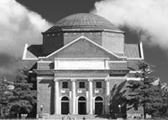
\includegraphics[width=0.6\linewidth]{hall_gray}
                        \caption{\texttt{hall\_gray}}
                    \end{subfigure}
                    \begin{subfigure}{\textwidth}
                        \centering
                        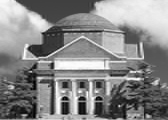
\includegraphics[width=0.6\linewidth]{hall_gray_rightzero}
                        \caption{右四列置零}
                    \end{subfigure}
                    \begin{subfigure}{\textwidth}
                        \centering
                        
\includegraphics[width=0.6\linewidth]{hall_gray_leftzero}
                        \caption{左四列置零}
                    \end{subfigure}
                    \caption{左右置零-整体图像测试结果}
                    \label{fig:rlzero}
                \end{figure}

            \item 若对\texttt{DCT}系数分别做转置、旋转\texttt{90}度和旋转\texttt{180}度操作,逆变换后恢复的图像有何变化?

                \begin{itemize}
                    \item \textbf{转置}使得行列频率信息交换,则逆变换后\textbf{图像被转置}

                        \[
                            \mathbf{C}^T = (\mathbf{DPD}^T)^T = \mathbf{DP}^T\mathbf{D}^T
                        \]

                        \begin{minted}{matlab}
>> A = hall_gray(97:104,153:160);
>> transpose = @(A)(A.');
>> I = imidct(imdct(A,transpose));
>> imwrite(I,'images\test_block_transpose.png');
                        \end{minted}

                        \begin{figure}[H]
                            \centering
                            \begin{subfigure}{0.5\textwidth}
                                \centering
                                
\includegraphics[width=0.6\linewidth]{test_block}
                                \caption{\texttt{test\_block}}
                            \end{subfigure}%
                            \begin{subfigure}{0.5\textwidth}
                                \centering
                                
\includegraphics[width=0.6\linewidth]{test_block_transpose}
                                \caption{转置}
                            \end{subfigure}
                            \caption{转置\texttt{DCT}系数}
                        \end{figure}

                    \item \textbf{旋转\texttt{90}度}使得直流分量系数变为纵向高频分量系数,则逆变换后\textbf{整体图像变暗,纵向高频分量强烈}

                        \begin{minted}{matlab}
>> I = imidct(imdct(A,@rot90));
>> imwrite(I,'images\test_block_rot90.png');
>> 
>> I = imidct(imdct(hall_gray,@rot90));
>> imwrite(I,'images\hall_gray_rot90.png');
                        \end{minted}

                        \begin{figure}[H]
                            \centering
                            \begin{subfigure}{0.5\textwidth}
                                \centering
                                
\includegraphics[width=0.6\linewidth]{test_block}
                                \caption{\texttt{test\_block}}
                            \end{subfigure}%
                            \begin{subfigure}{0.5\textwidth}
                                \centering
                                
\includegraphics[width=0.6\linewidth]{test_block_rot90}
                                \caption{逆时针旋转\texttt{90}度}
                            \end{subfigure}
                            \begin{subfigure}{0.5\textwidth}
                                \centering
                                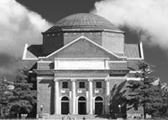
\includegraphics[width=0.6\linewidth]{hall_gray}
                                \caption{\texttt{hall\_gray}}
                            \end{subfigure}%
                            \begin{subfigure}{0.5\textwidth}
                                \centering
                                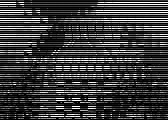
\includegraphics[width=0.6\linewidth]{hall_gray_rot90}
                                \caption{逆时针旋转\texttt{90}度}
                            \end{subfigure}
                            \caption{\texttt{DCT}系数逆时针旋转\texttt{90}度}
                        \end{figure}

                        纵向高频分量过强导致了明显的黑白分层,原有图像轮廓还能分辨,细节很难辨认。

                    \item \textbf{旋转\texttt{180}度}使得直流分量系数变为横纵高频分量系数,则逆变换后\textbf{整体图像变暗,横纵高频分量均变强}

                        \begin{minted}{matlab}
>> rot180 = @(A)(rot90(A,2));
>> I = imidct(imdct(A,rot180));
>> imwrite(I,'images\test_block_rot180.png');
>> 
>> I = imidct(imdct(hall_gray,rot180));
>> imwrite(I,'images\hall_gray_rot180.png');
                        \end{minted}

                        \begin{figure}[H]
                            \centering
                            \begin{subfigure}{0.5\textwidth}
                                \centering
                                
\includegraphics[width=0.6\linewidth]{test_block}
                                \caption{\texttt{test\_block}}
                            \end{subfigure}%
                            \begin{subfigure}{0.5\textwidth}
                                \centering
                                
\includegraphics[width=0.6\linewidth]{test_block_rot180}
                                \caption{旋转\texttt{180}度}
                            \end{subfigure}
                            \begin{subfigure}{0.5\textwidth}
                                \centering
                                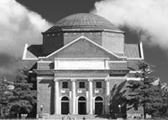
\includegraphics[width=0.6\linewidth]{hall_gray}
                                \caption{\texttt{hall\_gray}}
                            \end{subfigure}%
                            \begin{subfigure}{0.5\textwidth}
                                \centering
                                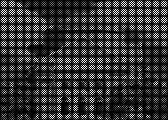
\includegraphics[width=0.6\linewidth]{hall_gray_rot180}
                                \caption{旋转\texttt{180}度}
                            \end{subfigure}
                            \caption{\texttt{DCT}系数旋转\texttt{180}度}
                        \end{figure}

                        强烈的横纵高频分量导致了明显的黑白分块,原有图像轮廓能凭借先验知识分辨,细节很难辨认。

                \end{itemize}

            \item 如果认为差分编码是一个系统,请绘出这个系统的频率响应,说明其滤波器类型。\texttt{DC}系数先进行差分编码再进行熵编码,说明\texttt{DC}系数的哪种分量更多?

                差分编码系统:

                \[
                    \hat{c}_D(n) = \left\{ \begin{matrix*}[l]
                        \tilde{c}_D(n) & n = 1 \\
                        \tilde{c}_D(n-1) - \tilde{c}_D(n) & elsewhere \\
                    \end{matrix*}
                    \right.
                \]

                不妨认为$\tilde{c}_D(n)$是因果信号,则差分编码系统传递函数为

                $$
                    H(z) = z^{-1} - 1
                $$

                是\textbf{高通滤波器},幅频特性如图\ref{fig:freqz_differential_coding}

                这说明\texttt{DC}系数中的\textbf{低频分量更多},通过差分编码滤去大量低频分量再进行熵编码,码长缩短。直观地说,\texttt{DC}系数中相邻系数一般相差不大,差分后压缩性能更佳。

                \begin{figure}[H]
                    \centering
                    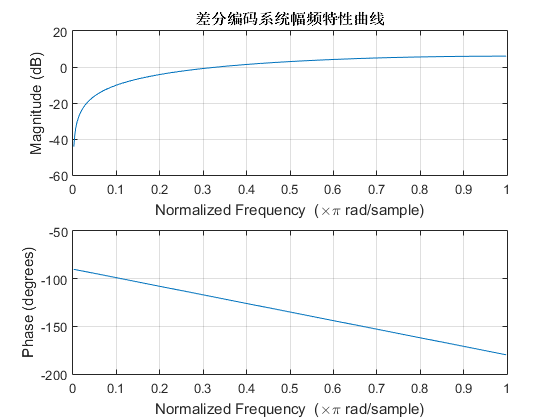
\includegraphics[width=\textwidth]{freqz_differential_coding}
                    \caption{差分编码系统幅频特性}
                    \label{fig:freqz_differential_coding}
                \end{figure}

            \item \texttt{DC}预测误差的取值和\texttt{Category}值有何关系?如何利用预测误差计算出其\texttt{Category}?

                观察表\ref{tab:DC_Huffman}容易得出:(预测误差记为\texttt{Error})

                $$
                    Error \in \{ 2^{Category-1} \leq \left| n\right| < 2^{Category} \mid n \in \mathbb{Z} \}
                $$

                $$
                    Category = \left \lceil \log_2{\left| Error \right| + 1} \right \rceil
                $$

            \item 实现\texttt{Zig-Zag}扫描

                \begin{figure}[H]
                    \centering
                    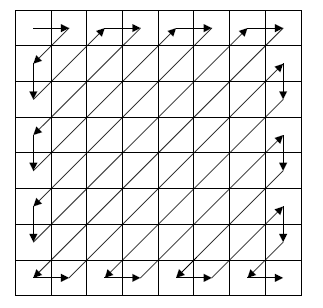
\includegraphics[width=0.5\textwidth]{Zig-Zag}
                    \caption{\texttt{Zig-Zag}扫描示意图}
                    \label{fig:zig_zag}
                \end{figure}

                \begin{enumerate}
                    \item 循环实现
                        \inputminted{matlab}{../zigzag1.m}
                        \begingroup
                            \captionof{listing}{\texttt{zigzag1.m}}
                        \endgroup

                    \item 查表实现:扫描固定$8\times 8$大小的矩阵可直接用查表法实现

                        \begin{listing}[H]
                            \caption{\texttt{zigzag2.m}}
                            \inputminted{matlab}{../zigzag2.m}
                        \end{listing}

                \end{enumerate}

                能想到的只有通用但低效的循环算法以及专用高效的查表法,在当前给定条件下,显然查表法更具有优势。

            \item 对测试图像分块、\texttt{DCT}和量化,将量化后的系数写成矩阵的形式,其中每一列为一个块的\texttt{DCT}系数\texttt{Zig-Zag}扫描后形成的列矢量,第一行为各个块的\texttt{DC}系数。

                先延伸图像使得其宽高像素值均为\texttt{8}的倍数,再分块、\texttt{DCT}、量化、\texttt{Zig-Zag}扫描,最后进行整合。

                \inputminted{matlab}{../quantize.m}
                \begingroup
                    \captionof{listing}{\texttt{quantize.m}}
                \endgroup

            \item 实现本章介绍的\texttt{JPEG}编码,输出为\texttt{DC}系数的码流、\texttt{AC}系数的码流、图像高度和图像宽度,写入\href{run:../result/jpegcodes.mat}{\texttt{jpegcodes.mat}}文件。

                \inputminted{matlab}{../jpeg.m}
                \begingroup
                    \captionof{listing}{\texttt{jpeg.m}}
                \endgroup

            \item 计算压缩比(输入文件长度/输出码流长度),注意转换为相同进制。

                压缩比$=\frac{height\times width\times 8}{length(DC\_stream) + length(AC\_stream)}=\frac{120\times168\times 8}{2031+23072}=6.42$

            \item 请实现本章介绍的\texttt{JPEG}解码。

                \textbf{思路:}

                \begin{enumerate}
                    \item 解\texttt{DC}码流:利用\texttt{DCTAB}逐行匹配得到\texttt{magnitude}码长,进一步解出系数;
                    \item 解\texttt{AC}码流:利用\texttt{ACTAB}逐行匹配得到\texttt{Run}、\texttt{Size},注意\texttt{EOB}和\texttt{ZRL}需特殊处理,进一步解出系数;
                    \item 逆\texttt{Zig-Zag}:查表法;
                    \item 反量化;
                    \item 按块逆\texttt{DCT}变换;
                    \item 拼接,\texttt{+128};
                    \item 裁剪图像使得与原图像宽高相同。
                \end{enumerate}

                \inputminted{matlab}{../dejpeg.m}
                \begingroup
                    \captionof{listing}{\texttt{dejpeg.m}}
                \endgroup

                \textbf{编解码效果:}

                \begin{enumerate}
                    \item \texttt{PSNR}评价:
                        \begin{minted}{matlab}
>> jpeg(hall_gray,QTAB,DCTAB,ACTAB);
>> load('result\jpegcodes.mat')
>> image = dejpeg(DC_stream,AC_stream,height,width,QTAB,DCTAB,ACTAB);
>> psnr = 10*log10(255^2/mse(image,hall_gray))

psnr =

   34.8926
                        \end{minted}

                        $PSNR=34.89dB$说明失真较小,编解码效果很好。

                    \item 主观评价:
                        \begin{figure}[H]
                            \centering
                            \begin{subfigure}{0.5\textwidth}
                                \centering
                                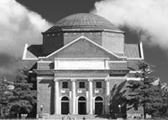
\includegraphics[width=0.6\linewidth]{hall_gray}
                                \caption{原图:\texttt{hall\_gray}}
                            \end{subfigure}%
                            \begin{subfigure}{0.5\textwidth}
                                \centering
                                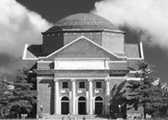
\includegraphics[width=0.6\linewidth]{hall_gray_dejpeg}
                                \caption{编解码后:\texttt{hall\_gray\_dejpeg}}
                            \end{subfigure}
                            \caption{主观评价编解码效果}
                        \end{figure}

                        肉眼几乎无法分辨编解码后图像与原图的区别,而压缩比达到了\texttt{6.42},这说明\texttt{JPEG}编码是十分有效的图像压缩编码。

                \end{enumerate}

            \item 将量化步长减小为原来的一半,重做编解码。

                \begin{minted}{matlab}
>> jpeg(hall_gray,QTAB/2,DCTAB,ACTAB);
>> load('result\jpegcodes.mat')
>> image = dejpeg(DC_stream,AC_stream,height,width,QTAB/2,DCTAB,ACTAB);
>> psnr = 10*log10(255^2/mse(image,hall_gray))

psnr =

    37.3208
                \end{minted}

                而可求得压缩比$=4.41$。

                由此可知,减小量化步长可进一步减小失真率,但也伴随着压缩比的迅速衰减。而标准量化步长可较好地兼顾图像质量与压缩比。

            \item 看电视时偶尔能看到美丽的雪花图像(\href{../resource/snow.mat}{\texttt{snow.mat}}),对其进行编解码。

                \textbf{预测:}\texttt{JPEG}编码利用了自然图像通常高频分量较少的特点,而美丽的雪花图像高频分量非常强(横纵方向黑白相间),可以预见\textbf{压缩比将大打折扣}。高频分量量化步长较大会导致\textbf{失真率升高}。

                \begin{minted}{matlab}
>> [DC_stream,AC_stream,height,width] = jpeg(snow,QTAB,DCTAB,ACTAB);
>> image = dejpeg(DC_stream,AC_stream,height,width,QTAB,DCTAB,ACTAB);
>> psnr = 10*log10(255^2/mse(image,snow))

psnr =

   29.5614

>> r = height*width*8/length([DC_stream,AC_stream])

r =

    3.6450
                \end{minted}

                结果符合预期,原因在预测部分已说明。

                \begin{figure}[H]
                    \centering
                    \begin{subfigure}{0.5\textwidth}
                        \centering
                        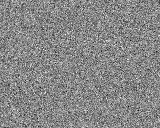
\includegraphics[width=0.6\linewidth]{snow}
                        \caption{原图:\texttt{snow}}
                    \end{subfigure}%
                    \begin{subfigure}{0.5\textwidth}
                        \centering
                        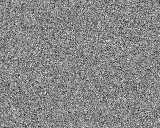
\includegraphics[width=0.6\linewidth]{snow_dejpeg}
                        \caption{编解码后:\texttt{snow\_dejpeg}}
                    \end{subfigure}
                    \caption{美丽的雪花图像编解码效果}
                \end{figure}

        \end{enumerate}
    
    % section 图像压缩编码 (end)

    

\end{document}